\documentclass{article}

\usepackage{graphicx}
\usepackage{hyperref}

\hypersetup{
    colorlinks=true,
    linkcolor=blue,
    filecolor=magenta,
    urlcolor=blue,
    pdftitle={Assignment 2},
    pdfpagemode=FullScreen,
}

\title{Assignment 2}
\author{Game Development with Unreal Engine}
\date{}

\begin{document}
\maketitle

\section*{Introduction}
This will be your second assignment. You have to work with the \verb|Widget Blueprint| and material parameters to create a simple user interface that allows you to change a material's parameters at runtime.

\section*{Environment}
Create a simple environment that supports your story. 

\section*{Interactions}
You'll have to figure out how to communicate between the widget blueprint and material parameters. This comes under blueprint communication and I've written a bit about these in the second part of my notes for week 2.

\section*{Hints}
This is a little tricky to do, so, some hints:
\begin{itemize}
    \item You can access the materials of a mesh in your blueprints by using the \verb|Get Material| node. To change a parameter, you need this material to be \emph{dynamic}, find a node that does this.
    \item Your system should work when there are multiple instances of the same blueprint in the world. I'll give a hint for this after a few days.
\end{itemize}

\section*{My attempt}
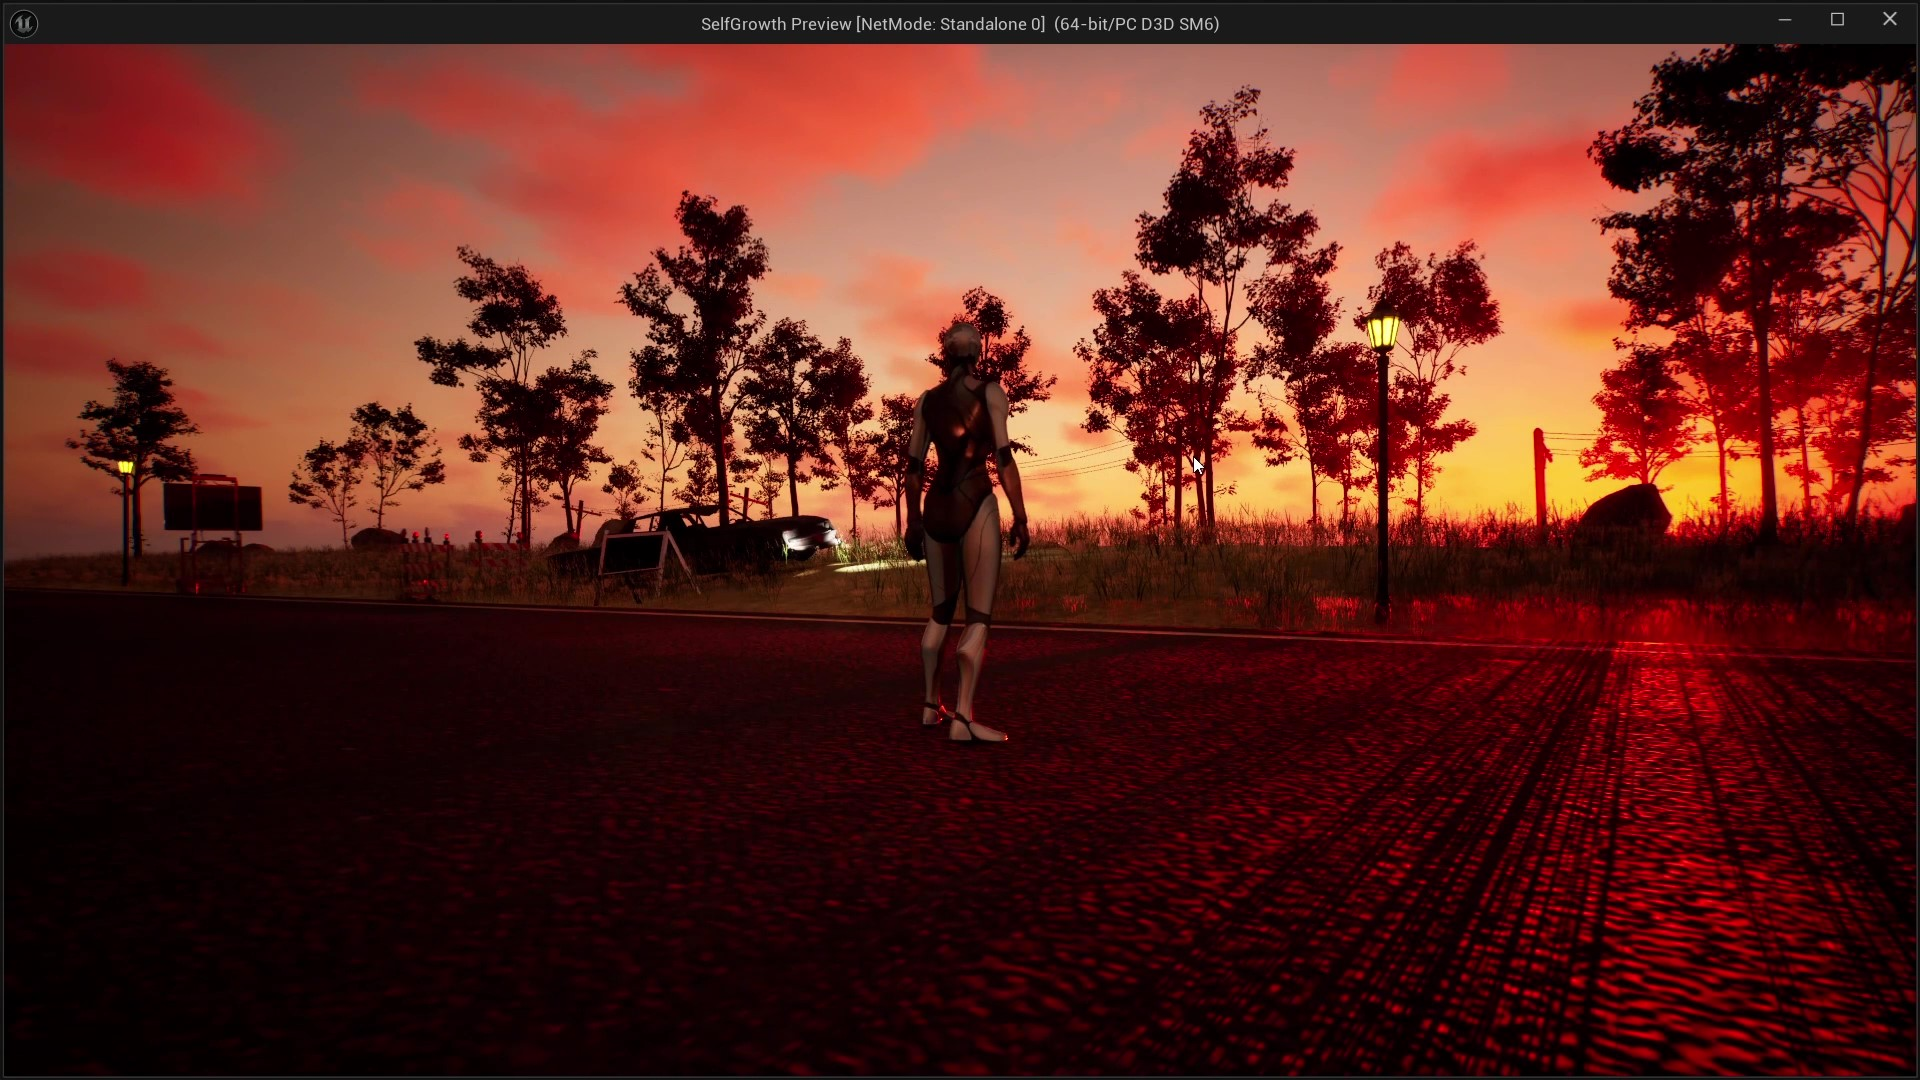
\includegraphics[width=\textwidth]{assn2images/image.jpg}
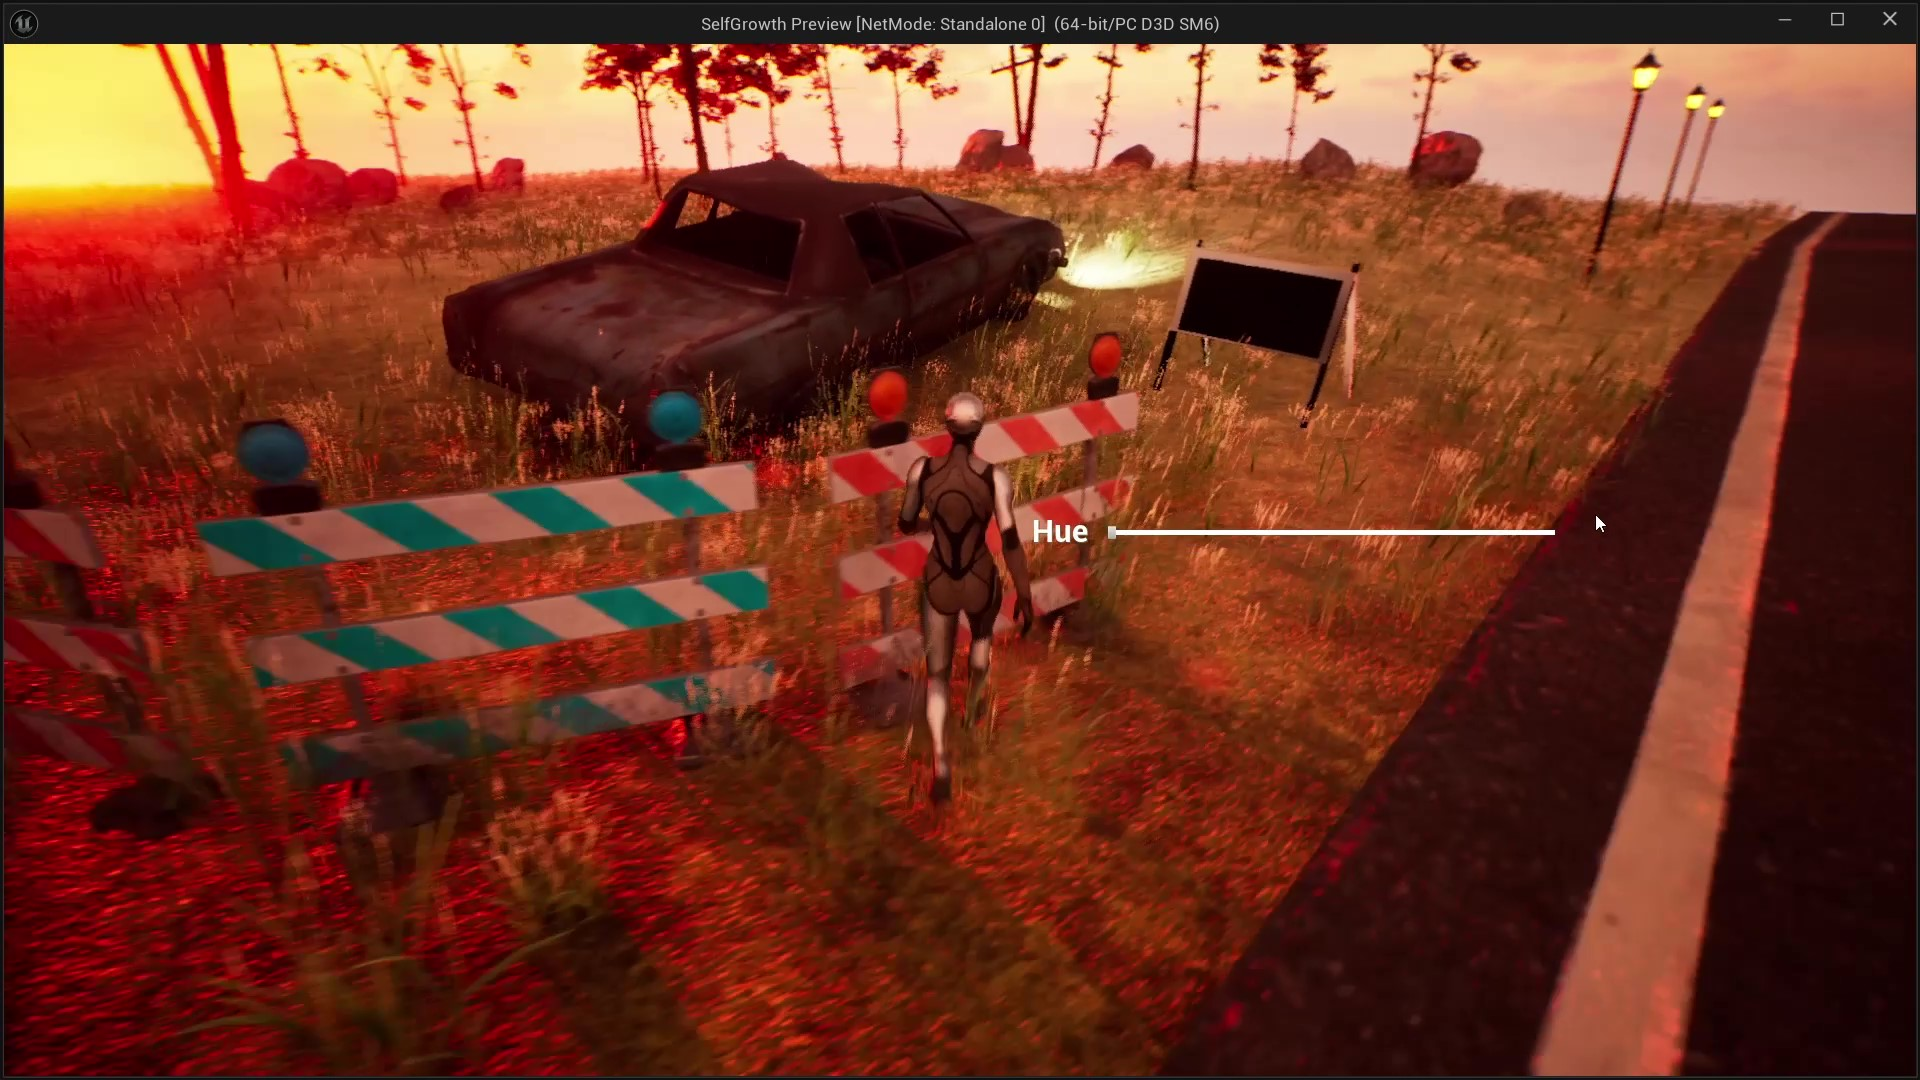
\includegraphics[width=\textwidth]{assn2images/image1.jpg}

The demo video can be found \href{https://drive.google.com/file/d/1P66idw2XpFjDfBoq9aDA1YSETFn0wb3c/view?usp=sharing}{here}.\\

I created three interfaces.
\begin{itemize}
    \item One allowed me to change the brightness of the street lights.
    \item One allowed my control over the headlights of the car.
    \item One allowed me to change the hue of the barriers.
\end{itemize}

\end{document}